\section{Arbeitsablauf des Schlussfolgerers}

In der nachfolgenden Abbildung \ref{image-u2r3-workflow} ist der gewöhnliche Ablauf des Reasoner dargestellt. Dabei ist er in drei Phasen einzuteilen. Das Laden der Ontologie, der Schlussfolgerungsvorgang und die Abfrage .

\begin{figure}
	\caption{Arbeitsablauf des Schlussfolgerers}
	\label{image-u2r3-workflow}
\begin{center}
	\scalebox{0.6}{
		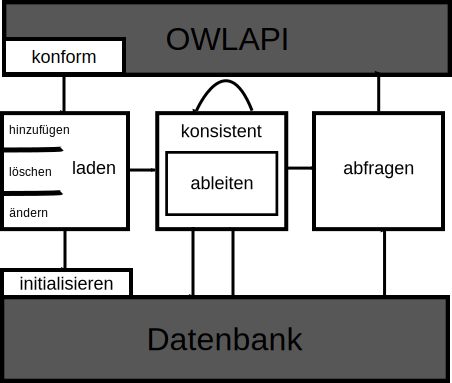
\includegraphics{images/u2r3-workflow.pdf}
	}
\end{center}
\end{figure}

\subsection{Konformität}
Konformität: überprüft, ob die verwendete Syntax im OWL2 RL Profil liegt
laden: bringt die Ontolgoie in das Datenbank-Schema, dabei merkt es an welche Regeln für das ableiten ausgeführt werden sollen
initialisieren: erzeugt das Datenbankschema notfalls, läd Standardwerte und richtet in der Datenbank nötige Funktionen ein
konsistent: ist eine Hülle um dafür zu sorgen, das nur über konsistente Fakten geschlossen wird. Die Häufigkeit kann eingestellt werden.
ableiten:Wendet die Ableitungsregeln an. Die Regelandwendung ist abgschloßen wenn keine neuen Fakten erzeugt werden können.
abfragen: implementiert die Schnittstelle der OWLAPI, mit der man Anfragen an die abgeleiteten Fakten stellen kann

\subsection{OWLAPI Anbindung}

Der obere Teil ist die sogenannte OWLAPI. Die OWLAPI ist eine Bibliothek die das Auslesen von Ontologien in verschiedenen Formaten erlaubt und eine Schlussfolgererschnittstelle für andere Programme zur Verfügung stellt. Durch die Implementierung dieser Schnittstelle in U2R3 ist es für alle Programme zugänglich die mit der OWLAPI arbeiten.
Die Schnittstelle stellt dabei auch eine Liste typischer Abfragen für einen Reasoner dar und kann allein dadurch schon als Messlatte für die Fähigkeiten eines Schlussfolgerers verwendet werden. Das OWLAPI-Projekt ist open-source und in Java implementiert und ist damit auch optimal für die Implementierung von U2R3 geeignet. Neben der reinen Parsertätigkeit kann die OWLAPI auch noch helfen zu überprüfen, ob eine Ontologie im OWL2 RL Profil liegt und nimmt damit weitere Arbeit ab.

\subsection{Das Laden einer Ontologie}

Die Inhalte einer Ontolgie die für das Schlussfolgern wichtig sind, sind die Axiome. Axiome sind dabei Fakten die als allgemein gültig angenommen werden. Sie dienen dazu das Universum der Ontologie zu modellieren und einen Startpunkt für weitere Schlussfolgerungen zu erzeugen.

Alle Axiome werden entsprechend dem MEMA-Prinzip abgelegt. Dabei ist für jedes Axiom genau eine Relation vorgesehen. Falls die Ontologie nicht OWL2 RL konform ist müssen für gewisse Axiome implizite Informationen abgelegt, wie. z.B.

\begin{table}
	\caption{Eine implizite Regel}
	\label{rule-impl}
\begin{center}
	\begin{tabular}{l|l}
    If & then \\ \hline
	T(?i1, ?property, ?i2 ) & T(?property owl:type ObjectProperty) \\
   \end{tabular}
\end{center}
\end{table}


\begin{verbatim}
* Wie wandelt man die Ontologie in INSERTs um?
* Wie läd man eine Ontologie?
\end{verbatim}


Falls ein Axiom aus komplexen Ausdrücken zusammengesetzt ist werden die Ausdrücke rekursiv abgearbeitet und einzeln behandelt. Zum herstellen der Beziehungen bei komplexen Axiomen werden Platzhalter für die Ausdrücke verwendet. Die Platzhalter die dabei erzeugt werden stammen von der OWLAPI aus der NodeID Klasse und folgen damit dem selben Schema wie auch bei anonymen Individuen.

In folgendem Besipeil soll der komplexe Ausdruck $A \sqcap \exists p.B \sqsubseteq C$ abgespeichert werden. Zur Verdeutlichung wurden Klammern eingebaut.

\begin{equation}
\overbrace{
	(\overbrace{A \sqcap (
		\overbrace{\exists{}p.B}
		^{nid3 \Rightarrow someValuesFrom(nid3, p, B)})}
	^{nid2 \Rightarrow intersectionOf(nid1, nid2), list(nid2, A, nid3)})}
^{nid1 \Rightarrow subClass(nid1, C)} \sqsubseteq C
\end{equation}

Wenn Fakten in eine Relation geschrieben werden, wird von dieser ein Hinweis (\emph{Reason}) an den Regelprozessor geschickt.

Dieser überprüft die Ursache und legt entsprechende Regeln an, die auf diese Veränderung ausgeführt werden können.

Die abzuarbeitenden Regeln enthalten eine Referenz auf die Fakten, die hinzugekommen sind. Allgemein sind sie so implementiert, das sie nur auf diesen neuen Fakten arbeiten -  auf den sogenannten Deltas - dies ist allerdings nicht in allen Fällen möglich (\emph{cls-int1}), sinnvoll (zu viele verschiedene Kombinationsmöglichkeiten) oder einfach zu komplex und damit fehleranfällig (\emph{prp-spo2}). Falls zwei oder mehrmals eine Regel auf die selben neuen Fakten erzeugt wird bevor sie ausgelöst wird, werden die beiden Regeln zu einer zusammengefasst und können je nach Einstellung neu priorisiert werden.

All diese Regeln sind in einer Warteschleife abgelegt, die beim Laden der Ontologie gefüllt wird und beim Abarbeiten, d.h. dem Realisieren, der Ontologie ausgelesen wird.

Regeln können durch das Erzeugen von neuen Fakten Hinweise für den Regelprozessor geben der daraufhin weitere Regeln anlegt und in die Warteschlange einsortiert.

Der Vorgang des Realisierens ist abgeschlossen, wenn keine Regel neue Fakten und damit neue Regeln erzeugen kann.

Der OWL2 RL Regelsatz garantiert dabei, das es immer zu einem Ende der Regelanwendung kommen wird, egal ob eine gültige oder ungültige Ontologie geladen wird.

Für das Abarbeiten und Erzeugen der Regeln ist hauptsächlich der Regelprozessor verantwortlich. Hier sind noch weitere Einstellungsmöglichkeiten, wie z.B. die parallele Verarbeitung von Regeln vorhanden.


\subsection{Das Schlussfolgern in einer Ontologie}
Das Schlussfolgern in einer Ontologie besteht darus die möglichen Regeln der OWL2 RL SPzeifiaktion anzuwenden. Diese Regeln erzeugen neue Fakten oder überpürfen dieKonsistenz. Der Schlussfolgerer hat seine Arbeit erledigt, wenn keine Regel neue Fakten erzeugen kann, Das sicherzustellen und dabei möglichst wenige Regeln anzuwenden ist seine Aufgabe. Daher wird im folgenden äher beschrieben, wann welche Regeln ausgelöst werden und in welcher Rehenfolge sie angewendet werden.

\subsubsection{Auswertungsstrategien}
Die Auswertungstrategie beschreibt in welcher Reihenfolge der Regelprozessor die Anwendung von Regeln auslöst. 

Der naive Ansatz wäre alle Regeln nacheinander auszuführen, d.h. alles Regeln die implementiert sind anwenden, wenn eine der Regeln dabei neue Fakten erzeugt muss dieser Vorgang wiederholt werden. Dieses Vorgehen ist trotz seiner leichten Umsetzbarkeit nicht implementiert, da der Reasoner damit unnötig viel Arbeit verrichten müssste.

Ein etwas fortgeschrittener Ansatz ist es die Abhängigkeiten der Regeln auszunutzen, d.h. nur wenn für die Prämisse einer Regel überhaupt Fakten vorhanden sind kann diese ausgelöst werden. Das heißt im konkreten, wenn eine Relation die in einer Regel in der Prämisse verwendet wird neue Daten enthält, dann muss diese Regel ausgelöst werden. Dieses Verfahren ist im Schlussfolgerer so umgesetzt.

Es wurde allerdings diese Vorgehen noch etwas weiter verbessert. Veränderungen in verschiedenen Tabellen könnten mehrmals die selbe Regel auslösen, da die Regel mehrere Vorbedingungen  hat. Die Regel wird dann nicht mehrfach ausgelöst sondern es werden erst alle Regeln in eine Warteschlange gesammelt. Wird eine neue Regel ausgelöst wird dann zuerst geschaut, ob diese Regel schon in der Warteschlange vorhanden ist.

Außerdem gibt es hier noch eine Optimierungsmöglichkeit, mit der man noch experimentieren kann. Wenn eine Regel in der Warteschlange erneut eingereiht werden soll, kann man sich entscheiden, ob die Regel an ihrere Stelle in der Schlange verbleibt oder ob sie herausgenommen wird und wieder ans Ende gestellt. Welches der beiden Verfahren besser ist muss sich erst noch in der Praxis zeigen.

In der Konfiguration des u2r3 ist diese Einstellungsmöglichkeit unter dem Namen \emph{EvaluationStrategy} zu finden. Gültige Werte dafür sind \emph{COMMONLAST} oder \emph{RARELAST}

\subsubsection{Regelauslösung}
Für jede Manipulation der Datenbank (DELETE/INSERT) wird eine Reason ausgelöst. Es wird dabei nur eine Reason ausgelöst, egal wieviele Zeilen von der Manipulation betroffen waren. Eine Reason löst dann weitere Actions aus, je nachdem welche Regeln davon betroffen sind.

\begin{verbatim}
DB Manipulation (1) ===> (1) Reason (1) ===> (n) RuleActions
\end{verbatim}


\begin{verbatim}
           Realtion                     Delta
            ######
            ######         <===           #
            ######
                                          |
(welche Regel) |                          | (welche neuen Daten)
               |                          |
                ####>  Reason  <==========

                          | (1)
                          |
                          | (eine Regel mit neuen Daten)
                          |
                          v (n)

                      RuleAction
\end{verbatim}


\subsection{Das Abfragen einer Ontologie}
Das Abfragen in einer Ontologie lässt sich grundlegend in zwei Arten aufteilen. Erstens man hat einen AUsdruck und möchte überpürfen, ob dieser geschlussfolgert worden ist. Diese Art von Abfrage liefert nur a oder nein zurück. Die zweite Art von Abfrage möchte eine ERgebnismenge zurück. Dabei ist im Gegensatz zur ersten Art von Abfrage eine Variable in der Abfrage, die gefüllt wird.

Bei beiden ist grundsätzlich so, dass das ``Anfrage'' OWL-Konstrukt in eine SQL-ABfrage umgeformt wird. In beiden Fällen kann die Abfrage beantwortet werden egal on die SQL-ABfrage etwas zurückbringt oder nicht.. Im zweiten Fall muss aber bei einem Ergebnis daraus noch eine Ergebnis ereugt werden, so das es dem OWLAPI Format entspricht.

\section{Komplexe Ausdrücke}
Was sind komplexe Ausdrücke?
\subsection{Komplexe Ausdrücke finden}
Einfügen von Statements oder Werten nicht gut, weil darüber nicht geschloßen werden kann bzw. wenn darüber Aussagen gemacht werden sollen muss erst geschloßen werden. (zeitaufwendig!)
